\documentclass[10pt, a4paper]{article}
\usepackage{graphicx} 
\usepackage{multicol}
\usepackage{enumitem}
\usepackage{float}
\usepackage[left=25mm, top=20mm, right=25mm, bottom=20mm, nohead, footskip=15mm]{geometry}
\pagestyle{plain}
\setcounter{page}{279}

\title{ \textbf{Model of Interoperability of Information
Systems of Information and Communication
Environment of Secondary Special Education
Institution}}
\author{Nikolai Listopad and Lizaveta Bushchik\\
 \textit{Belarusian State University of Informatics and Radioelectronics}\\
Minsk, Belarus\\
Email: listopad@bsuir.by, e.bushchik@bsuir.by}
\date{}
\setlist{nolistsep}
\begin{document}
\maketitle
\begin{multicols}{2}
\textbf{\textit{Abstract}—The paper proposes a model of interoperability
of information systems of information and communication
environment of secondary vocational education institution.
It shows what should be understood under the interoperability of information systems in relation to the industry of
education on the example of secondary special education
institution. The system of business processes in the institution of specialized secondary education in the following
directions: controlling, operating (basic, describing the
educational process of the institution) and supporting is
presented. The author’s root model of business processes
of educational institution is given. The well-known reference
model of interoperability in the form of three levels -
organizational, semantic and technical - is specified and
supplemented by the parameters which were detailed for
the college. The three-level model of interoperability of
college information systems is refined on the basis of the
processor approach, which allowed creating a flexible and
adaptive management in the institution of secondary special
education. }
\par
\textbf{ \textit{Keywords}—digital transformation, interoperability, information and communication environment, process management}
\par
\begin{center}
  I. Introduction
\end{center}

At present, information systems, different in their composition, parameters and characteristics, are developing
towards their integration and globalization. The term
unified information space, which is understood as the
interaction of various information systems for the exchange and use of information under common protocols,
standards and rules, sounds more and more often. In
this case, such knowledge-intensive areas as economics,
industry, and defense are mainly analyzed.
\par
Digital transformation, in the new era of digital economy, is impossible without the creation and development
of a heterogeneous information and communication environment, the transparency of which is ensured through
the use of open systems principles. One of the most
important features of such open systems is interoperability, which is understood as the ability of systems and
components to interact (exchange information and use
the information obtained from the exchange), based on
the use of information and communication technologies
(ICT) [1], [2]. The main property of interoperability
is the seamless information integration of individual
elements and systems as a whole. The relevance of
ensuring interoperability increases significantly with the
transition of all areas of ICT application (Fig. 1) to the
stage of digital transformation.
\begin{figure}[H]
  \includegraphics[width=\linewidth]{image1.png}
  \caption{Interoperability — a key requirement for different applications.}
\end{figure}
\par
All these domain areas should be seen as subsystems
of the information society, and not isolated, but closely
interacting. As it follows from the figure, the problem
of interoperability extends to such subsystems of the
information society as e-government, e-science, e-health,
e-education, e-businness and other areas, since virtually
no area of knowledge and economy can develop today
without the use of information and telecommunication
technologies. The process integration of socio-electronic
systems into the information society is carried out with
the help of the Industry 4.0 platform. The provision of
interoperability acts as one of the key factors of the
industrial concept of Industry 4.0, which also includes:
\begin{enumerate}
\item[1)]  Product Lifecycle Management (PLM) is the pro279
cess of managing a product at all stages, from
idea, design and production to sales, service and
withdrawal from the market.
\item[2)] Big Data is a variety of big data stored on digital
media.
\item[3)] SMART Factory — this concept provides a flexible
modular multi-platform production system with
a high level of informatization and visualization,
organized according to the principles of "lean
manufacturing".
\item[4)] Cyber-physical systems is a system consisting of
various physical entities of any kind, artificial
subsystems, such as various sensors and sensors,
and controllers, allowing to present such an entity
as a whole.
\item[5)] The Internet of Things (IoT) is a global computing network, combining various kinds of physical
objects, capable of interacting with each other and
the outside world [3].
\end{enumerate}
Industry 4.0 enables the creation of an efficient enterprise business model, where efficiency is achieved
primarily through the rational management of automation
systems for physical production operations and related
processes integrated into a single information space.
\par
Blockchain technology is crucial for the realization of
a single information space with interoperability in mind.
This decentralized, open-source technology allows the
creation of interoperable products between blockchains,
allowing more users, businesses and institutions to remain interconnected."
\par
One new technology in industrial automation is "smart
drones," which are unmanned aircraft with automatic or
remote control capabilities. They are used for various
purposes, including photo and video shooting, aerial
photography, aerial scanning, assessment of different
terrains, detection of security threats, field research, etc.
\par
The key area of e-government development is the
formation of the national information and educational
environment, which should ensure the consistent implementation of digital transformation processes and
their effective management. Transferability, interoperability and scalability should be the prerequisites for the
successful implementation of the national information
and educational environment.
\par
When solving the problems of interoperability, organizational changes aimed at the introduction of flexible
and adaptive information and education systems (IES) of
different levels in educational institutions are of primary
importance. The necessary flexibility in managing the
process of educational activity can be provided by the
process approach to its organization.
\par
The process management of educational institution in
this study is understood as an activity aimed at the
implementation of business processes with the highest
possible efficiency under given constraints (human, material, immaterial, financial resources) [4].
\par
To move to process management, it is necessary to formalize all business processes, determine which processes
are the most demanded and most effective, how they are
organized and how to control their effectiveness. The task
of formalization is always solved by the introduction of
a system of standards.
\par
Process standardization in this case is understood as
a set of measures, methods, tools and elements of the
organizational structure that ensures the development,
implementation, enforcement, maintenance and timely
cancellation of outdated regulatory and procedural documents of the organization [5].
\begin{center}
  II. Interoperability of information systems in
institutions of secondary special education
\end{center}
\par
Let’s consider interoperability in education on the
example of a specialized secondary education institution.
The activity of training specialists with specialized secondary education includes a system of business processes
represented in the form of the following areas:
\begin{itemize}
  \item \textit{controlling} — manage the functioning of the educational system of the educational institution;
  \item \textit{operational (basic)} — describe the educational process of the educational institution;
  \item \textit{supporting} — serve the main activities of the educational institution (Fig. 2).
\end{itemize}
\begin{figure}[H]
  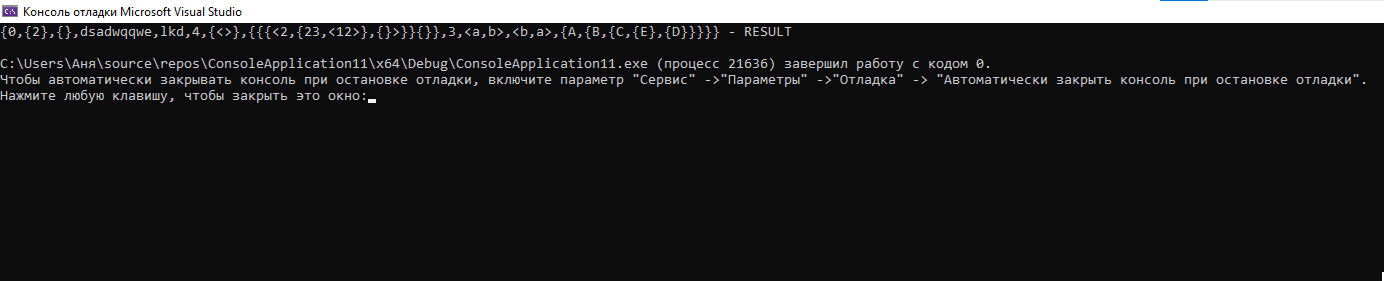
\includegraphics[width=\linewidth]{image2.png}
  \caption{Business processes of secondary special educational institution.}
\end{figure}
\par
These processes must be considered from a systemic
approach, i.e., their interconnection and mutual influence
on each other.The presented processes are basic, in
particular educational institutions new modules can be
added to them, new interrelations can be formed, so the
presented scheme is open.
\par
The implementation of the process approach must
begin with the construction of a ROOT MODEL of
business processes which are necessary for organizing
and managing the activities of an educational institution.
The ROOT MODEL of business processes is used to
compile a classifier of business processes, and also shows
the links between structural divisions, which allows at the
output of the model to correlate business processes with
structural divisions and their functions.
\par
The scheme of the root business process model is
shown in Figure 3.
\begin{figure}[H]
  \includegraphics[width=\linewidth]{image3.png}
  \caption{Root model of business processes of educational institution.}
\end{figure}
\par
The ROOT MODEL of business processes includes
three modules, each of which consists of generalized
business processes and reflects their relationship through
the flow of information.
\par
The main module is operational processes. They determine the educational vector of the educational institution:
the design of educational and program documentation,
planning the educational process, the training of specialists at the level of secondary special education, ideological and educational work, the distribution of graduates.
\par
The control processes module covers all business
processes and is mainly focused on planning processes,
whose activities are focused on providing educational
services in accordance with the requirements of society
and the state, which is the input data for the evaluation
and subsequent adjustment of the strategic and operational plans of the educational institution.
\par
The supporting processes module includes business
processes that provide conditions for effective functioning of operational processes.
\par
The result of the organized interconnected activity of
all modules is a specialist with specialized secondary
education. The root model of business processes can
further serve as the basis for the classifier of business
processes.
\par
To ensure the interoperability of the information system modules it is reasonable to develop a problemoriented interoperability model.
\par
To date, there are many different models describing the
interaction of information systems. In order to select a
basic model by analogy with the approach implemented
in the Russian Federation, let us distinguish four levels
of interoperability (Fig. 4):
\begin{enumerate}

  \item[1)] no interoperability;
  \item[2)] technical level;
  \item[3)] semantic level;
  \item[4)] the organizational level [6].
\end{enumerate} 
\par
Note that each level of interoperability should correspond to a set of standards and specifications, so that the
system developers could create a profile that includes a
set of harmonized standards from all the necessary levels.
\begin{figure}[H]
  \includegraphics[width=\linewidth]{image4.png}
  \caption{Basic levels of interoperability.}
\end{figure}
\par
The first level of the interoperability model — no interoperability — means that all communication between
information systems is done manually.
\par
Thus, the college interoperability model can be based
on the interoperability reference model presented in
GOST R 55062-2012. This model consists of three
levels: organizational, semantic, technical [7]. For each
of the levels the interoperability parameters have been
identified, which have been detailed to represent the
college interoperability model. To form the sublevels and
taking into account more parameters in the problemoriented model of the college information system, the
international experience of interoperability formalization,
presented in the SCOPE-model, can be used.
\par
As we know [8], SCOPE-model is designed for
qualitative-quantitative assessment of interoperability of
different aspects of the analyzed system at its different
levels, according to a certain set of parameters.
\par
Today there are many technologies for interoperability.
However, these tools are used in isolation from each
other and are not linked into a coherent methodological
system. All the many known approaches to solving
interoperability problems at the technological, semantic
and organizational levels can be roughly divided into the
following categories [8]:
\begin{enumerate}

  \item[1)] bottom-up approach (bottom-up approach), which
focuses primarily on solving the problems of technological interoperability of information systems
by using common standards and technologies for
transmitting, storing, representing and processing
information at all levels of integration of these
systems;
  \item[2)] top-down approach (top-down approach), which
focuses on the decomposition of the solution of
interoperability problems from the perspective of
the system architecture as a whole, and then from
the perspective of individual subsystems and processes down to atomic elements;
  \item[3)]  system-wide approach, based on the analysis of internal communications between components within
\end{enumerate} 
\end{multicols}



\end{document}
